\documentclass{beamer}
\mode<presentation>
\usepackage{amsmath,amssymb,mathtools}
\usepackage{textcomp}
\usepackage{gensymb}
\usepackage{adjustbox}
\usepackage{subcaption}
\usepackage{enumitem}
\usepackage{multicol}
\usepackage{listings}
\usepackage{url}
\usepackage{graphicx} % <-- needed for images
\def\UrlBreaks{\do\/\do-}

\usetheme{Boadilla}
\usecolortheme{lily}
\setbeamertemplate{footline}{
  \leavevmode%
  \hbox{%
  \begin{beamercolorbox}[wd=\paperwidth,ht=2ex,dp=1ex,right]{author in head/foot}%
    \insertframenumber{} / \inserttotalframenumber\hspace*{2ex}
  \end{beamercolorbox}}%
  \vskip0pt%
}
\setbeamertemplate{navigation symbols}{}

\lstset{
  frame=single,
  breaklines=true,
  columns=fullflexible,
  basicstyle=\ttfamily\tiny   % tiny font so code fits
}

\numberwithin{equation}{section}

% ---- your macros ----
\providecommand{\nCr}[2]{\,^{#1}C_{#2}}
\providecommand{\nPr}[2]{\,^{#1}P_{#2}}
\providecommand{\mbf}{\mathbf}
\providecommand{\pr}[1]{\ensuremath{\Pr\left(#1\right)}}
\providecommand{\qfunc}[1]{\ensuremath{Q\left(#1\right)}}
\providecommand{\sbrak}[1]{\ensuremath{{}\left[#1\right]}}
\providecommand{\lsbrak}[1]{\ensuremath{{}\left[#1\right.}}
\providecommand{\rsbrak}[1]{\ensuremath{\left.#1\right]}}
\providecommand{\brak}[1]{\ensuremath{\left(#1\right)}}
\providecommand{\lbrak}[1]{\ensuremath{\left(#1\right.}}
\providecommand{\rbrak}[1]{\ensuremath{\left.#1\right)}}
\providecommand{\cbrak}[1]{\ensuremath{\left\{#1\right\}}}
\providecommand{\lcbrak}[1]{\ensuremath{\left\{#1\right.}}
\providecommand{\rcbrak}[1]{\ensuremath{\left.#1\right\}}}
\theoremstyle{remark}
\newtheorem{rem}{Remark}
\newcommand{\sgn}{\mathop{\mathrm{sgn}}}
\providecommand{\abs}[1]{\left\vert#1\right\vert}
\providecommand{\res}[1]{\Res\displaylimits_{#1}}
\providecommand{\norm}[1]{\lVert#1\rVert}
\providecommand{\mtx}[1]{\mathbf{#1}}
\providecommand{\mean}[1]{E\left[ #1 \right]}
\providecommand{\fourier}{\overset{\mathcal{F}}{ \rightleftharpoons}}
\providecommand{\system}{\overset{\mathcal{H}}{ \longleftrightarrow}}
\providecommand{\dec}[2]{\ensuremath{\overset{#1}{\underset{#2}{\gtrless}}}}
\newcommand{\myvec}[1]{\ensuremath{\begin{pmatrix}#1\end{pmatrix}}}
\newcommand{\mydet}[1]{\ensuremath{\begin{vmatrix}#1\end{vmatrix}}}

\newenvironment{amatrix}[1]{%
  \left(\begin{array}{@{}*{#1}{c}|*{#1}{c}@{}}
}{%
  \end{array}\right)
}

\newcommand{\myaugvec}[2]{\ensuremath{\begin{amatrix}{#1}#2\end{amatrix}}}
\let\vec\mathbf
% ---------------------

\title{Matgeo Presentation - Problem 10.7.104}
\author{ee25btech11056 - Suraj.N}

\begin{document}

\begin{frame}
  \titlepage
\end{frame}

\begin{frame}{Problem Statement}

Let \(a,b\) and \(\lambda\) be positive real numbers. Suppose \(P\) is an end point of the latus rectum of the parabola \(y^2=4\lambda x\), and suppose the ellipse \(\dfrac{x^2}{a^2}+\dfrac{y^2}{b^2}=1\) passes through the point \(P\). If the tangents to the parabola and the ellipse at the point \(P\) are perpendicular to each other, then the eccentricity of ellipse is 

\end{frame}

\begin{frame}{Data}

\begin{table}[h!]
  \centering
  \begin{tabular}{|c|c|}
\hline
\textbf{Name} & \textbf{Value} \\
\hline
Circle & $\vec{x}^\top\vec{x} - a^2 = 0$ \\
\hline
Line & $\vec{x} = \myvec{\tfrac{a}{\sqrt{2}} \\ 0} + \kappa\myvec{0 \\ 1}$ \\
\hline
\end{tabular}

  \caption*{Table : Parabola and Ellipse}
  \label{10.7.104}
\end{table}

\end{frame}

\begin{frame}{Solution}

The parameters of the parabola are :

\begin{align}
  \vec{V_1} &= \myvec{0 & 0\\0 & 1} & \vec{u_1} &= \myvec{-2\lambda\\0} & f_1 &= 0
\end{align}

The parameters of the ellipse are :

\begin{align}
  \vec{V_2} &= \myvec{\tfrac{1}{a^2} & 0\\0 & \tfrac{1}{b^2}} & \vec{u_2} &= \vec{0} & f_2 &= -1 \label{eq:ellipse} 
\end{align}

The end point of the latus rectum of parabola is 

\begin{align}
  \vec{P} &= \myvec{\lambda\\2\lambda}
\end{align}

\end{frame}

\begin{frame}{Solution}

The equation of tangent to the parabola at $\vec{P}$ is given as :

\begin{align}
  (\vec{V_1}\vec{P}+\vec{u_1})^\top\vec{x} + \vec{u_1}^\top\vec{P} + f_1 &= 0 & \vec{n_1} &= \vec{V_1}\vec{P}+\vec{u_1} 
\end{align}

The equation of tangent to the ellipse at $\vec{P}$ is given as :
\begin{align}
  (\vec{V_2}\vec{P}+\vec{u_2})^\top\vec{x} + \vec{u_2}^\top\vec{P} + f_2 &= 0 & \vec{n_2} &= \vec{V_2}\vec{P}+\vec{u_2} 
\end{align}
As the tangents at $\vec{P}$ are perpendicular , the normal vectors of the tangents are also perpendicular 
\begin{align}
  \vec{n_1}^\top\vec{n_2} = 0\\
  (\vec{V_1}\vec{P}+\vec{u_1})^\top\vec{V_2}\vec{P} = 0\\
  (\vec{P}^\top\vec{V_1}^\top+\vec{u_1}^\top)\vec{V_2}\vec{P} = 0\\
  \myvec{-1 & 1}\myvec{\tfrac{1}{a^2} & 0\\0 & \tfrac{1}{b^2}}\myvec{1\\2} = 0\\
  \frac{a^2}{b^2} = \frac{1}{2} \label{eq:ab} 
\end{align}

\end{frame}

\begin{frame}{Solution}

From \eqref{eq:ellipse} , the eigen values of $\vec{V_2}$ are the diagonal entries as it is an upper triangular matrix and also $a<b$

\begin{align}
  \lambda_1 &= \frac{1}{b^2} & \lambda_2 &= \frac{1}{a^2}
\end{align}

The eccentricity e of ellipse is given as 

\begin{align}
  e = \sqrt{1 - \frac{\lambda_1}{\lambda_2}}\\
  e = \sqrt{1 - \frac{a^2}{b^2}}
\end{align}

From \eqref{eq:ab} , we get 

\begin{align}
  e = \frac{1}{\sqrt{2}}
\end{align}

\end{frame}

\begin{frame}{Plot}

\begin{figure}[h!]
  \centering
  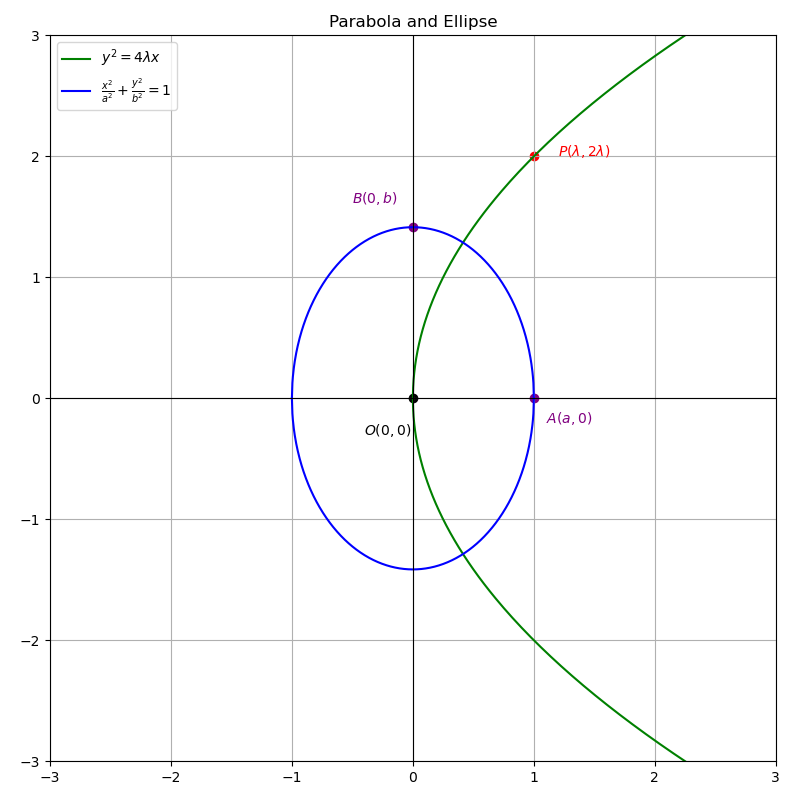
\includegraphics[width=0.6\columnwidth]{figs/parabola_ellipse.png} 
   \caption*{Fig : Parabola and Ellipse}
  \label{Fig1}
\end{figure}

\end{frame}

\end{document}

